\usepackage{geometry}
\usepackage{times}
\usepackage{DejaVuSansMono}
\usepackage{geometry}
 \geometry{
 % total={7.2in,9.6in},
 % left=0.65in,
 % top=0.8in,
   margin=0.6in
}
\usepackage[utf8,applemac]{inputenc}
\usepackage{etaremune}
\usepackage{enumitem}
\usepackage[numbers]{natbib}

\usepackage{xcolor,color}
\usepackage[hyphens]{url}
\urlstyle{same}
\usepackage[hyphenbreaks]{breakurl}
\usepackage[colorlinks=true,linkcolor=myblue,citecolor=myblue,urlcolor=myblue]{hyperref}
\definecolor{myblue}{RGB}{0,0,170}
\usepackage[compact]{titlesec}
\newcommand{\hruleafter}[1]{
  #1
  \hrule height .5pt
  \vspace{-.2in}
}

%% bibliography with multiple entries
\usepackage[resetlabels,labeled]{multibib}
\newcites{thes,prep,undr,jrnl,conf,tech,invt,pres,selected}{{ },{ },{ },{ },{ },{ },{ },{ },{ }}


\usepackage{fancyhdr}
\usepackage{lastpage}
\pagestyle{fancy}
\fancyhf{}
\renewcommand{\headrulewidth}{0pt}
\rhead{
  \flushleft
  Sungho Shin \hfill
  \thepage/\pageref{LastPage}
  \hrule
  \vspace{-.3in}
}

\makeatletter
\def\@maketitle{%
  \newpage
  \null
  \vspace{-.2in}
  \begin{center}%
    \let \footnote \thanks
    {\Large\bf \@title \par}%
    % \vskip 1em%
    % \lineskip .5em%
    % \begin{tabular}[t]{c}%
    %   \@author
    % \end{tabular}\par
    % \vskip 1em%
    % {\large \@date}%
  \end{center}%
  \par
  \vskip 1em}
\makeatother
\usepackage{multicol}
\usepackage{graphicx}


\titleformat{\subsection}{\large\bfseries}{\thesection}{}{\hruleafter}

%% reverse numbering of bibliography
\usepackage{etaremune,etoolbox}
\makeatletter
\AtBeginDocument{
  \renewenvironment{thebibliography}[1]
  {
    \begin{etaremune}[itemsep=0mm]
      \let\citeN\cite\let\shortcite\cite\let\citeasnoun\cite}
    {\bibitem@fin\bibpostamble
      \def\@noitemerr{\PackageWarning{natbib}{Empty `thebibliography' environment}}%
    \end{etaremune}
  }
}
  \renewcommand{\thebibliography}[1]{\oldbibliography{#1}
    } %Reducing spacing in the bibliography.
\patchcmd{\@lbibitem}{\item[\hfil\NAT@anchor{#2}{\NAT@num}]}{\item}{}{}
\makeatother

\let\oldbibliography\thebibliography
\renewcommand{\thebibliography}[1]{%
  \oldbibliography{#1}%
  \setlength{\itemsep}{0pt}%
}

\bibliographystyle{plain}

\begin{document}
\begin{tikzpicture}[align=center,font=\footnotesize]
  \node at (0,1) {
    Energy Infrastructures\\[.5em]
    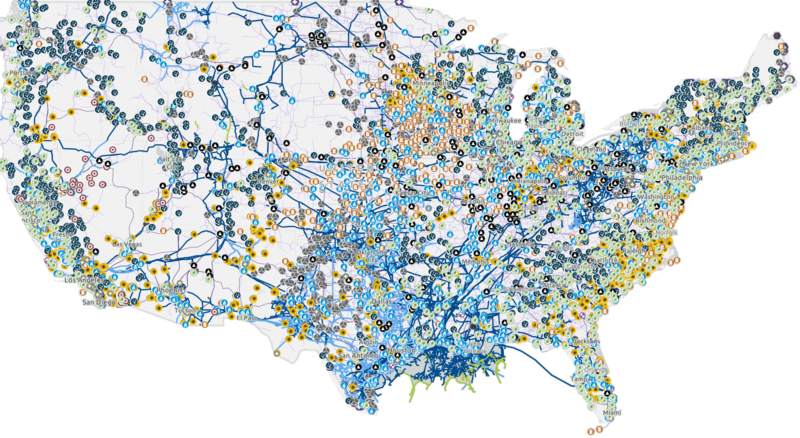
\includegraphics[width=200pt]{map-old.png}
  };
  \node at (0,-1.5) {
    Emerging Technologies
  };
  \node at (-2.7,-2.7) {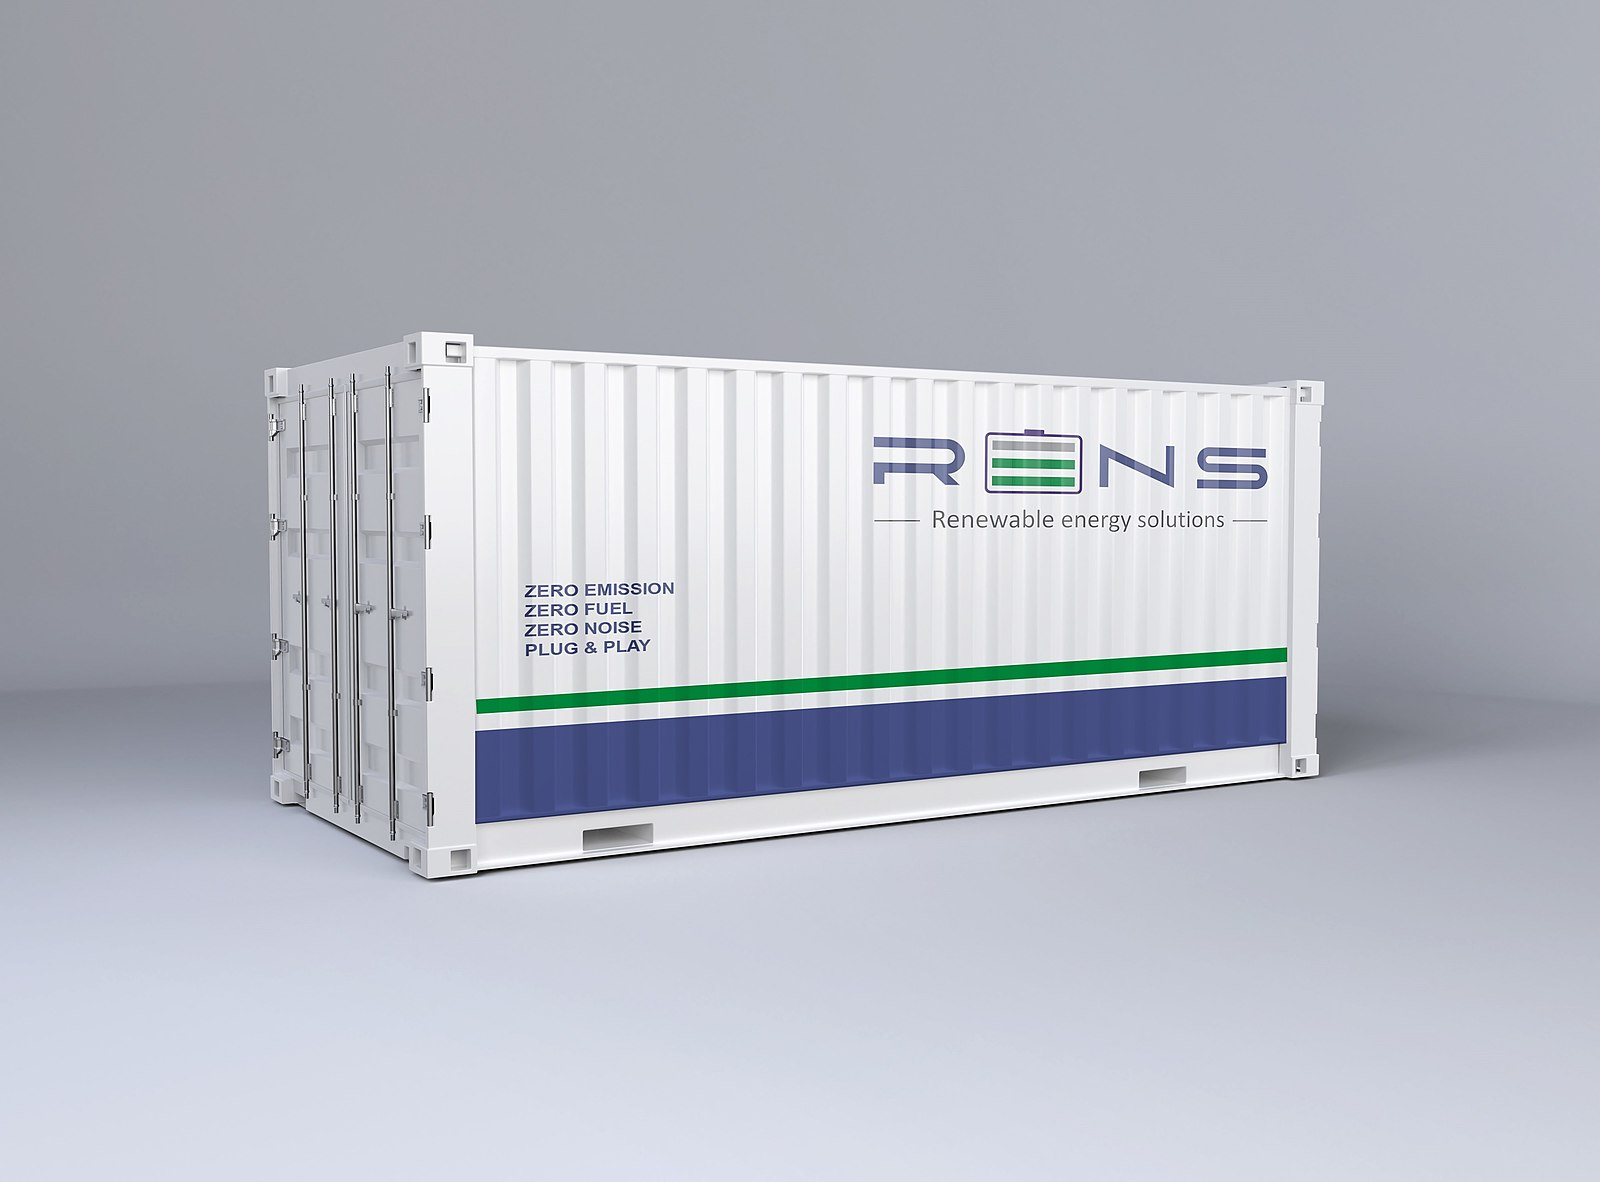
\includegraphics[width=76pt,height=46pt]{battery.jpg}};
  \node at (0,-2.7) {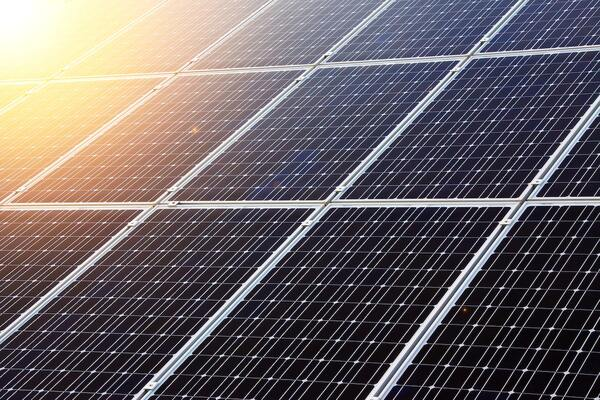
\includegraphics[width=76pt,height=46pt]{solar.jpg}};
  \node at (2.7,-2.7) {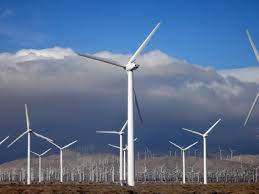
\includegraphics[width=76pt,height=46pt]{wind.jpg}};
  \node at (-2.7,-4.35) {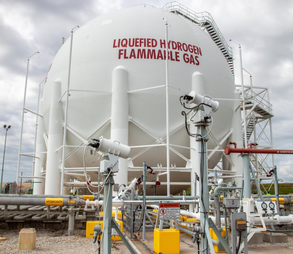
\includegraphics[width=76pt,height=46pt]{hydrogen.png}};
  \node at (0,-4.35) {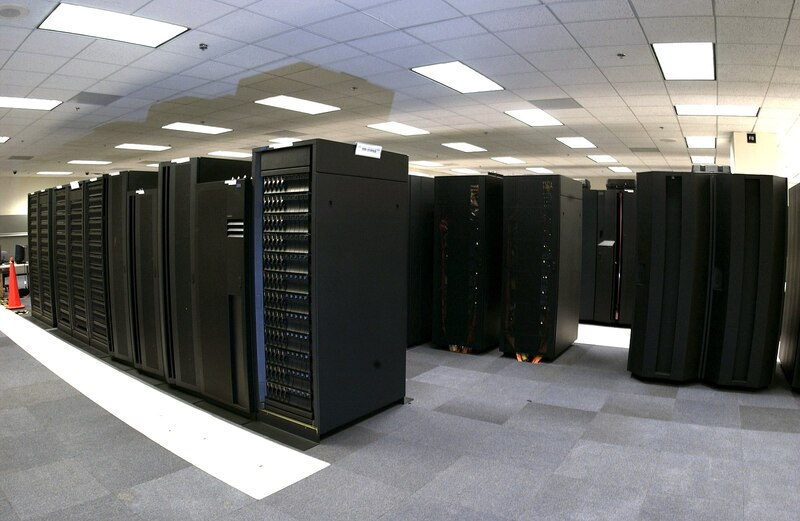
\includegraphics[width=76pt,height=46pt]{data-center.jpg}};
  \node at (2.7,-4.35) {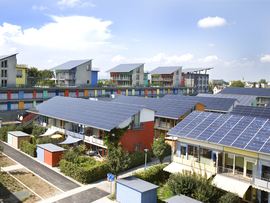
\includegraphics[width=76pt,height=46pt]{microgrid.jpg}}; 
  \draw[-latex] (2,-.25) to [in=45, out=-45] node[right] {Interactions} (2,-1.5);
  \draw[-latex] (-2,-1.5) to [out=135, in=-135] node[left] {Interactions} (-2,-.25);s
\end{tikzpicture}
\end{document}
